%-------------------------- Algorithm~\ref{LT_1} --------------------------------------------------------------------------------------
\begin{algorithm}[t]
\fontsize{8}{9.6} \selectfont
\DontPrintSemicolon
\KwIn{Digraph $G = \{V, A\}$ \break Vertices Set $V = \{Candidate, Mine\}$ \break Arcs Set $A = \forall a \in A, R_{a}^2 > Threshold_{R^2}$       }
\KwOut{Lower and Upper Bounds of Circuit Lifetime}
\Begin{
$Vector~Vtr$\;
      \For{$\forall i \in Candidate$}
      {
          \For{ $\forall p \in V, p \neq i, \exists a \in A$, $a$ is the arc from $i$ to $p$}{
          $LT_{p}$ = Estimate $p's$ lifetime based on binary search\;
          \If{ $LT_{p} < Smallest$}{  $Smallest =  LT_{p}$}
          }
        }
        Put $Smallest$ into $Vtr$ \;
  }
  \KwRet{Smallest value in $Vtr$, largest value in $Vtr$}
\caption{Lifetime Interval Estimation of Designs\label{LT_1}}
\end{algorithm}
%-------------------------- Algorithm~\ref{LT_2} -------------------------------------------------------------------------------------
\begin{algorithm}[t]
\fontsize{8}{9.6} \selectfont
\DontPrintSemicolon
\KwIn{Modified netlist (after DCC insertion), critical path $p$ and critical path $i$ }
\KwOut{Lifetime of path $p$}
\Begin{
Upper Bound $U$\;
Lower Bound $L$\;
Median~$M$\;
	\While{ $U - L < 10^{-3}$}
	{	$M = \frac{U + L}{2}$ \;
		//Derive aging rate of path $i$ i.e., $X_{i}$. Path $i$ is assume undergo worst-case aging \;
		$X_{i} = A\times \alpha^{n} \times  t^{n}$\;
		//Predict $p's$ aging rate i.e., $Y_{p}$ by the regression of $p$ on $i$\;
		$Y_{p} = \alpha_{pi} \cdot$ $X_{i} + \beta_{pi}$\;
		$S_{p}$ = Estimate $p's$ slack considering an aging rate of $Y_{p}$\;
		\eIf{ $S_{p} > 0$}{  
			$L =  M$
		}{
			$U =  M$
		}
	}
\KwRet{$U$}
}
\caption{Path Lifetime Estimation based on Binary Search\label{LT_2}}
\end{algorithm}

%-------------------------- LT -------------------------------------------------------------------------------------
\section{LIFETIME ESTIMATION}
\label{sec:lt_estimation}
\begin{comment}
\begin{figure*}[!ht]
    \centering
    \subfigure{
    	\label{fig:sub:alg1}
        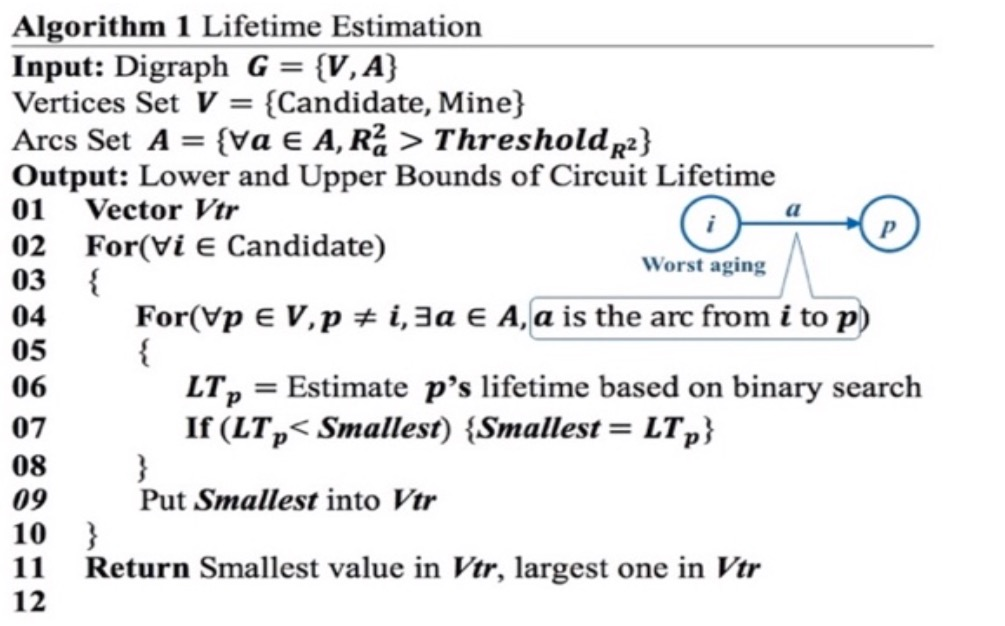
\includegraphics[width=0.9\columnwidth]{algorithm1.png}
    }
    \hspace{1.6cm}
    \subfigure{
    	\label{fig:sub:alg2}
        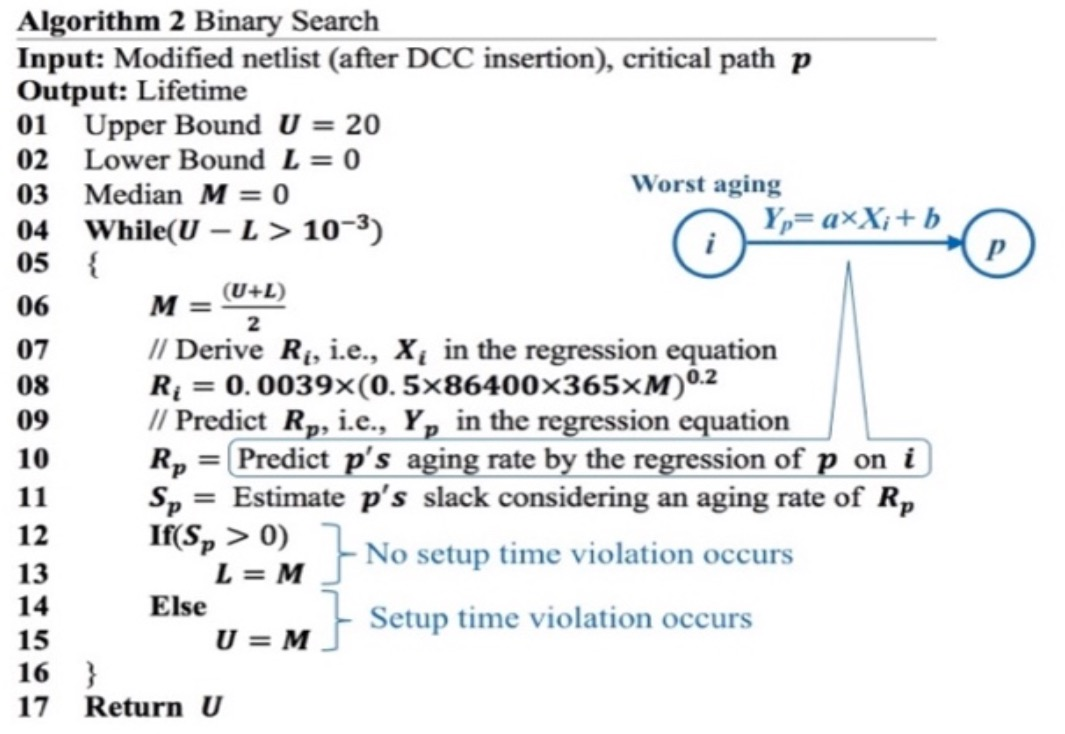
\includegraphics[width=0.8\columnwidth]{algorithm2.png}
    }
    \caption{Algorithms used to estimate lifetime of designs}
    \label{fig:en}
\end{figure*}
\end{comment}
%-------------------------- Paragraph --------------------------------------------------------------------------------------
In this section, we propose two algorithms to estimate the lifetime of design circuits, which is attacked by our proposed framework using DCCs, considering the workload variations (i.e., various operational modes) from users. 

It is worth reminding that the previous assumption, introduced in Section~\ref{sec:frame:mds}, says that the union of critical operational modes of all candidate paths is equivalent to the universe of operational modes. That is, after applying worst-case aging on each candidate path (Line 3 in Algorithm~\ref{LT_1}), all operational modes are considered, during the lifetime estimation in our methodology. Here, Line 2 in Algorithm~\ref{LT_1}, says that a candidate path $i$ is assumed to age in the worst case. Then, in the inner for-loop (Lines 4-8), we iteratively estimate the lifetime of other paths based on prediction from the worst-case aging of $i$. For each path, say $p$ (Line 4), the following steps are applied to estimate $p's$ lifetime: ($i$, Line 6) $p's$ lifetime can be estimated based on a binary search in Algorithm~\ref{LT_2} ($ii$, Line 7) the estimated lifetime is compared against the smallest one, since the smallest lifetime among all paths determines the circuit lifetime.
In Algorithm~\ref{LT_2}, path $p's$ lifetime is estimated based on a binary search. The upper/lower bounds for the binary search are set in Lines 1-2, respectively. In Line 6, M is set as the median value of two bounds; and in Line 10, $p's$ aging rate $Y_{p}$ is predicted by the regression equation of $p$ on $i$, 
\begin{equation*}
	\fontsize{8}{8} \selectfont
	Y_{p} = \alpha_{pi} \cdot X_{i} + \beta_{pi}
\end{equation*}
where $ \alpha_{pi}$ and $\beta_{pi}$ are coefficients, and path $i$ is assumed to age under M-year worst-case condition and its aging rate $X_{i}$ is derived by the following predictive model, which in presented in \cite{wang2007efficient}:
\begin{equation}
	\fontsize{8}{8} \selectfont
	A \cdot \alpha^n \cdot t^n 
	\label{eq:worst}
\end{equation}
where $A$ and $n$ are fitted constants, $\alpha$ denotes the stress duty cycle, and $t$ denotes time (unit is second). $\alpha$ is usually set to 0.5. $A$ and $n$ are fitted as 0.0039 and 0.2, respectively, after SPICE simulation.

Then, in Line 11, $Y_{p}$ is used to estimate $p's$ slack $S_{p}$, which is utilized to check whether the setup-time violations will occur on p under the aging rate $Y_{p}$ (Line 12). If the value of $S_{p}$ is negative, it denotes that, setup-time violations will occur on $p$ after M years at an aging rate of $Y_{p}$ (Line 14). Afterwards, according to result of the above timing check, the upper/lower bound for next iteration will be set in Line 13 or 15. While repeating the above steps (Lines 5-17), both bounds gradually converge. Eventually, the converged value of the upper bound is considered as $p's$ lifetime (Line 17), which will be returned to Algorithm 1 as the value of $LT_{p}$ (Line 6 in Algorithm~\ref{LT_1}).

The aforementioned procedures are repeated for each candidate path. We can derive a lifetime value by considering a specific candidate path. By considering all of the candidate
paths, all operational modes are considered and we can find a group of lifetime values, i.e., $V_{tr}$ in Algorithm~\ref{LT_1}. The smallest value and the largest one within $V_{tr}$ are the resulting lifetime interval found based on this given attack.